\subsection{Introduction}
Synchronized activity among neurons occurs in many brain areas and there are evidences
suggesting that it is relevant for information processing, especially sensory
processing, cognition, and sleep. Patters of reverberating synchronized activity are
believed to reflect neuronal representations of cognitive processes and stored
memories. Notice that this kind of synchronized activity is also observed
\textit{in vitro} in the form of reverberating synchronous activity.\\
Said so, a network burst (NB) can be described straightforward as a synchronized
bursting event involving most units of the network, thus implying that several
channels are exhibiting bursting activity at the same time.
\begin{figure}[H]
    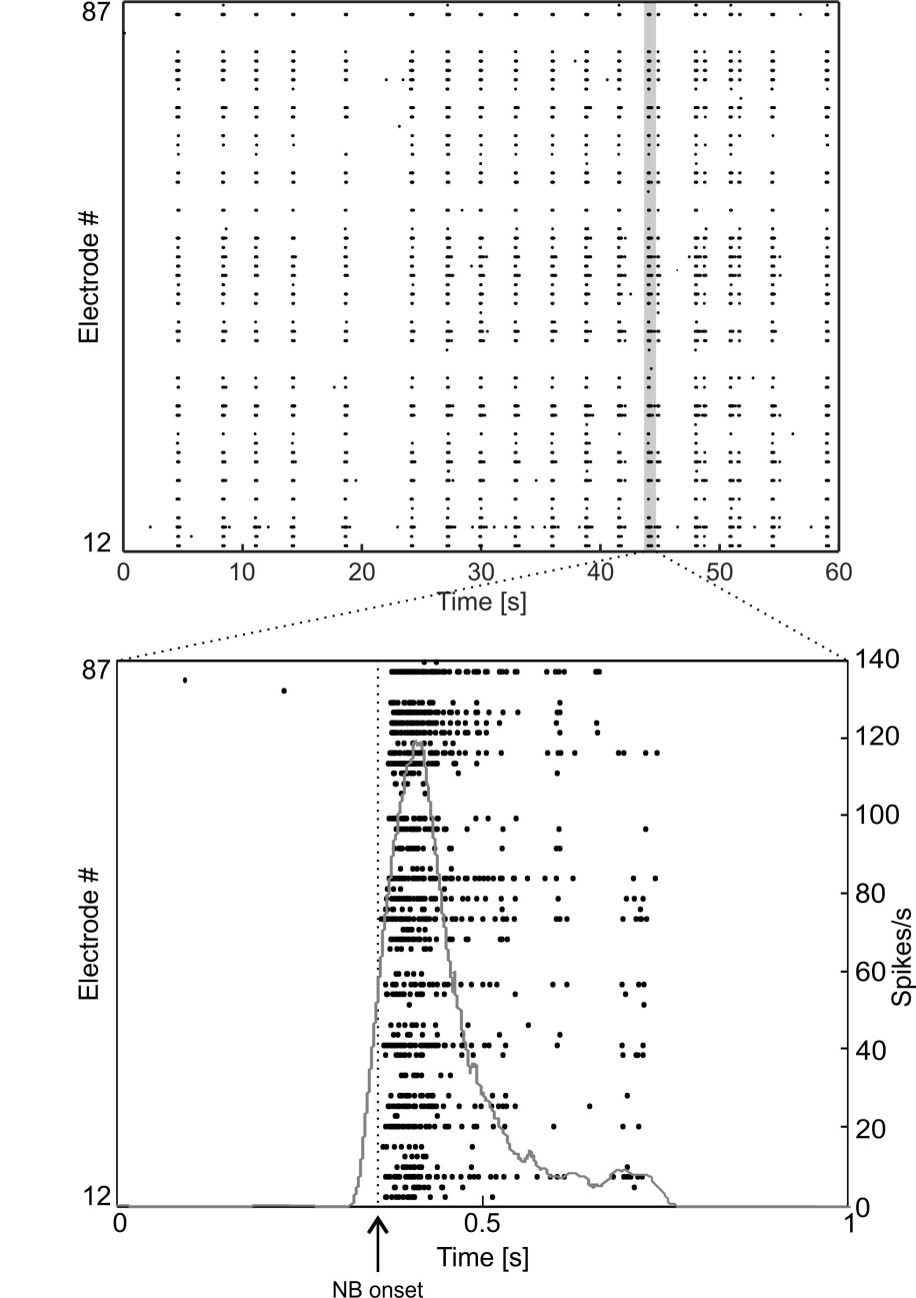
\includegraphics[scale=0.5]{7_1}
    \centering
\end{figure}
Let's point out that network bursting closely reminds to the \textit{UP} and
\textit{DOWN} states of the \textit{in vivo} cerebral cortex during slow-wave
sleep. In addition, spontaneous network bursting activity is also easily
noticed in developing brain, as it is thought to play a key role in
ontogeny - i.e. the origination and development of an organism -
of a neuronal network.
Moreover, let's recall that a strong correlation between the high frequency (spikes)
and low frequency (LFP) signals exists. Said so, it is possible to individuate mainly
6 types of waves, each one described by a typical frequency range:
\begin{itemize}
    \item Delta: \(0.5-4\,Hz\)
    \item Theta: \(4-8\,Hz\)
    \item Alpha: \(8-11\,Hz\)
    \item Beta: \(11-30\,Hz\)
    \item Low Gamma: \(30-55\,Hz\)
    \item High Gamma: \(55-80\,Hz\)
\end{itemize}

\subsection{Example: a step into sleep physiology}
In mammals and birds, sleeping activity is divided into pretty much different
phases, according to the characteristics exhibited by the brain activity.
\begin{itemize}
    \item \textbf{Rapid Eye Movement (REM):} this phase is also known as paradoxical
    sleep and its greatest peculiarities are the fact that eyes are rapidly moving
    and a rapid low-voltage EEG, akng to the awake state.
    \item \textbf{Non-Rapid Eye Movement (NREM):} this broad category keeps together
    all the phases where the neuronal activity is considerably different w.r.t. the
    awake state. NREM stages can be individuated according to the acivity differences:
    \begin{itemize}
        \item \textbf{N1:} it refers to the transition of the brain from alpha waves
        (awake state) towards theta waves, having a lower frequency. This stage is
        often called drowsy sleep.
        \item \textbf{N2:} it is characterized by a phenomenon denominated sleep
        spindles - i.e. bursts of activity - displaying a pretty higher frequency range
        (\(11-16\,Hz\)). Another typical phenomenon occurring in this stage is named
        K-complexes.
        \item \textbf{N3:} this stage is commonly denominated deep sleep and it is
        characterized by the presence of delta waves (at least \(20\%\) of the
        overall activity). Notice that delta waves exhibit especially high
        peak-to-peak voltages (\(>75\,\mu{V}\)).
        \item \textbf{N4:} this stage is usually described as a state in which slow
        delta waves overcomes the \(50\%\) threshold on the total brain oscillatory
        activity. It is sometimes considered together with stage N3.
    \end{itemize}
\end{itemize}
\begin{figure}[H]
    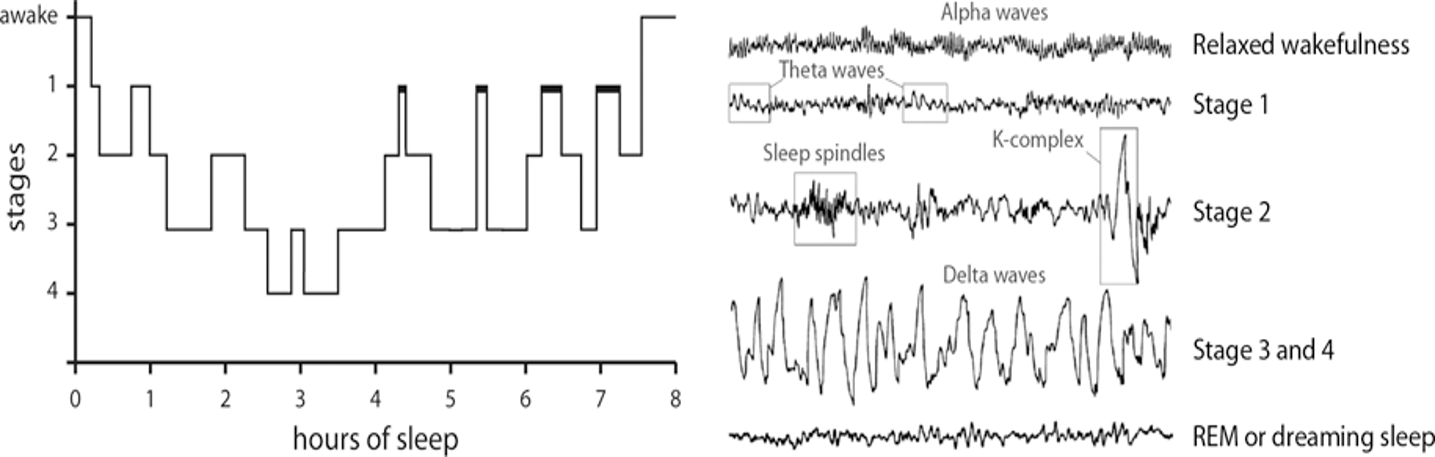
\includegraphics[scale=0.52]{7_2}
    \centering
\end{figure}
There is evidence that network bursting activity is strictly related to the delta
waves typical of deep sleep.

\subsection{Network Burst Detection}
In order to detect network burst, it is necessary to be able to recognize synchronous
increases in the network activity. A number of algorithms have been developed to
solve such a task.
\subsubsection{The Van Pelt algorithm}
Let's recall the definition of network bursts, as they are short episodes of
synchronized firing among many recording sites. Notice that network bursts are not
exclusively described by increased firing rates at individual sites, but also by an
increase of the number of active sites. This method consists in dividing the time
axis into a number of small bins and computing the product between the number of
active sites - i.e. the recording channels showing firing activity - and the total
number of spikes at these sites. In case of uncorrelated spiking activity among
the sites, this product won't significantly differ from the total spike count, however
it raise sharply as soon as the firing becomes synchronized. The time point at
which the previously illustrated product attains its maximal value is used to
define a center-of-mass-based time center of the network burst.
\begin{figure}[H]
    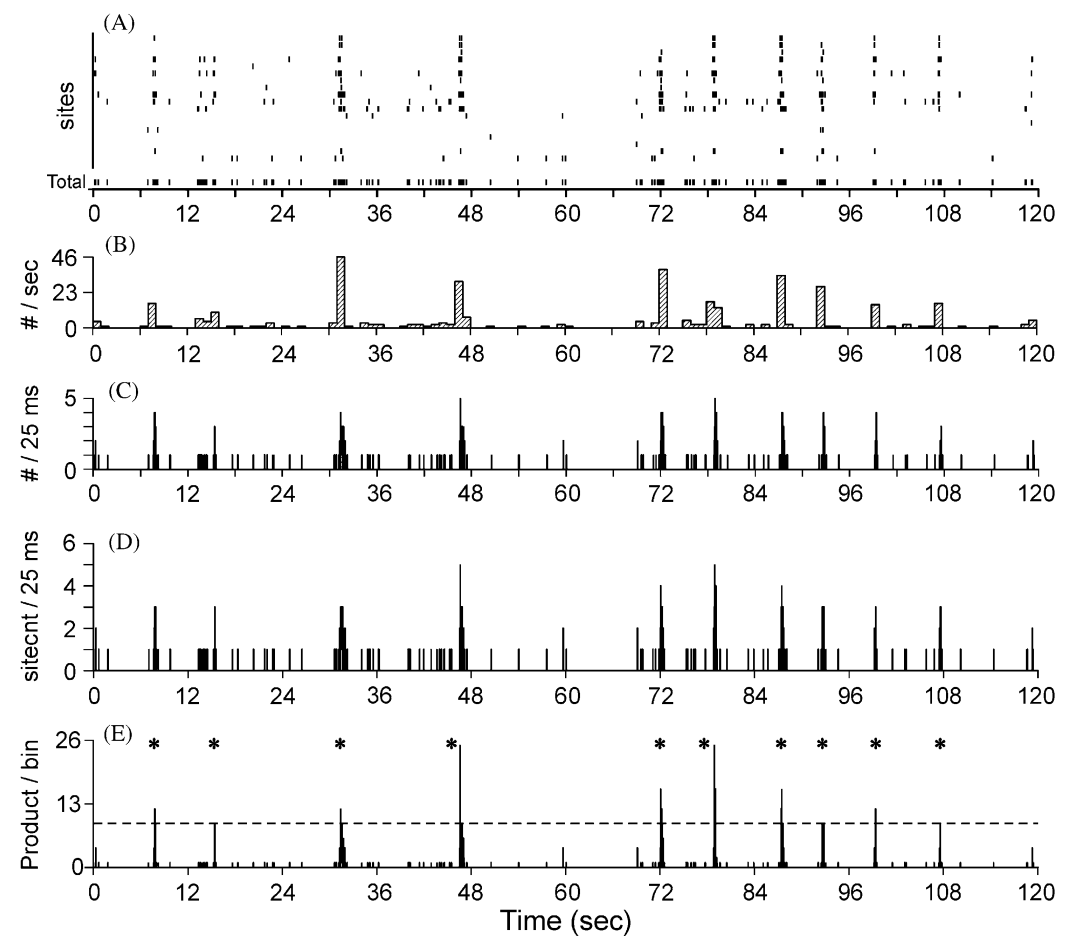
\includegraphics[scale=0.6]{7_3}
    \centering
\end{figure}
The figure above shows the following plots:
\begin{itemize}
    \item \textbf{(A)} The time points of spikes at the different recording sites of
    a multi-electrode array. The lowest trace shows the total spike train for all
    the sites.
    \item \textbf{(B)} A total network firing rate plot with time bins of \(1\,s\).
    \item \textbf{(C)} A total network firing rate plot with time bins of \(25\,ms\).
    \item \textbf{(D)} A plot of the number of active sites with time bins
    of \(25\,ms\).
    \item \textbf{(E)} A plot of the product of total number of spikes and the
    number of active sites, calculated per \(25\,ms\) time bins. The dashed line
    represents a threshold to overcome to identify an actual network burst, which
    are individuated by a star.
\end{itemize}
\subsubsection{The LogISI method}
This technique requires instead that burst detection has been performed for every
recording channel. Then, a burst event train for each channel is derived, where
bursts are described as single point events, disregarding every information about
their duration. These points for all the sites are then projected onto the same axis.
Now it is possible to perform once again burst detection on this new axis, allowing
to look for time periods with an increased bursting activity on several channels, thus
synchronized. This algorithm consists in an iterative application of burst detection
procedures. Notice that the minimum number of intra-burst spikes for the cumulative
burst event train can be intended as the minimum number of active channels required
to detect a network burst event, usually set as the \(20\%\) of the total number of
recording sites.
\begin{figure}[H]
    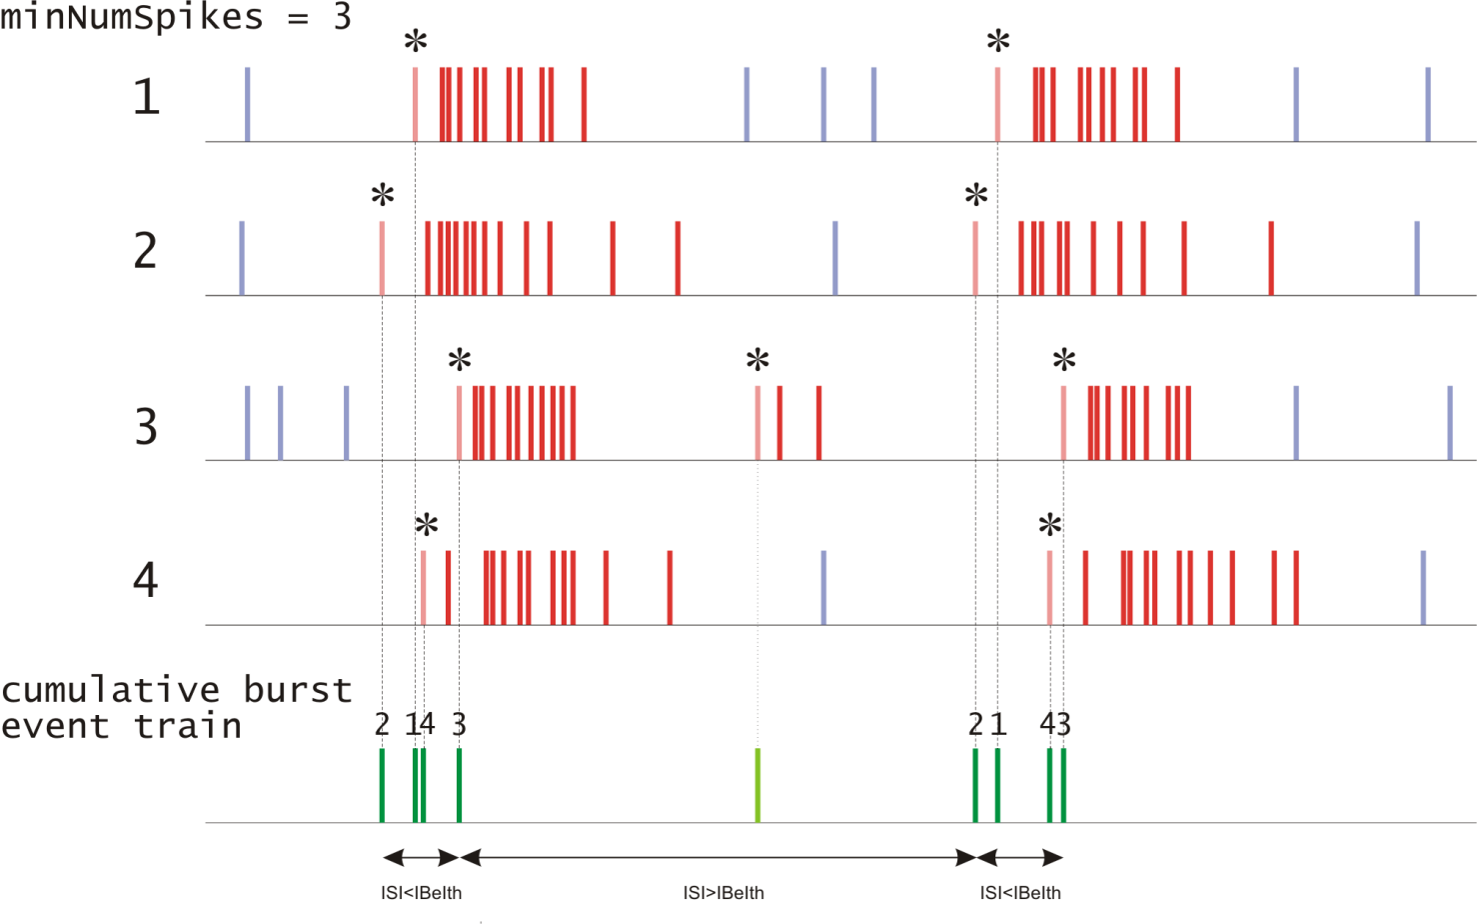
\includegraphics[scale=0.75]{7_4}
    \centering
\end{figure}

\subsection{Metrics}
Some of the most relevant metrics to characterize netowrk bursting are reported
in the following.
\subsubsection{The Burstiness Index}
The burstiness index (\(BI\)) metric was empirically derived by D. A. Wagenaar in order to assess the burstiness
of a neuronal network with just one number. From experiments, it has been notice that
in general the overall time occupied by network bursts in a whole recording is
always less than \(15\%\) of the total duration and this has been taken as an
assumption for the computation of constants employed to derive the burstiness
index. The computation steps are reported here:
\begin{enumerate}
    \item Divide a 5 minutes recording into 300 time bins (each 1 second long).
    \item Count the total number of spikes for each bin, across all the recording sites.
    \item Compute the fraction of the total number of spikes contained in the \(15\%\),
    of bins with the largest counts, indicated as \(f_{15}\).
    \begin{itemize}
        \item If the firing rate is tonic, then \(f_{15}\) is expected to be close to 0.15.
        \item If a recording is bursty, it is likely that most of the spikes will
        be contained in bursts, resulting in \(f_{15}\) close to 1.
    \end{itemize}
    \item Compute the burstiness index normalized between 0 and 1 as
    \begin{align*}
        BI = \frac{f_{15}-0.15}{0.85}
    \end{align*}
\end{enumerate}